% Options for packages loaded elsewhere
\PassOptionsToPackage{unicode}{hyperref}
\PassOptionsToPackage{hyphens}{url}
%
\documentclass[
]{book}
\usepackage{amsmath,amssymb}
\usepackage{lmodern}
\usepackage{iftex}
\ifPDFTeX
  \usepackage[T1]{fontenc}
  \usepackage[utf8]{inputenc}
  \usepackage{textcomp} % provide euro and other symbols
\else % if luatex or xetex
  \usepackage{unicode-math}
  \defaultfontfeatures{Scale=MatchLowercase}
  \defaultfontfeatures[\rmfamily]{Ligatures=TeX,Scale=1}
\fi
% Use upquote if available, for straight quotes in verbatim environments
\IfFileExists{upquote.sty}{\usepackage{upquote}}{}
\IfFileExists{microtype.sty}{% use microtype if available
  \usepackage[]{microtype}
  \UseMicrotypeSet[protrusion]{basicmath} % disable protrusion for tt fonts
}{}
\makeatletter
\@ifundefined{KOMAClassName}{% if non-KOMA class
  \IfFileExists{parskip.sty}{%
    \usepackage{parskip}
  }{% else
    \setlength{\parindent}{0pt}
    \setlength{\parskip}{6pt plus 2pt minus 1pt}}
}{% if KOMA class
  \KOMAoptions{parskip=half}}
\makeatother
\usepackage{xcolor}
\usepackage{color}
\usepackage{fancyvrb}
\newcommand{\VerbBar}{|}
\newcommand{\VERB}{\Verb[commandchars=\\\{\}]}
\DefineVerbatimEnvironment{Highlighting}{Verbatim}{commandchars=\\\{\}}
% Add ',fontsize=\small' for more characters per line
\usepackage{framed}
\definecolor{shadecolor}{RGB}{248,248,248}
\newenvironment{Shaded}{\begin{snugshade}}{\end{snugshade}}
\newcommand{\AlertTok}[1]{\textcolor[rgb]{0.94,0.16,0.16}{#1}}
\newcommand{\AnnotationTok}[1]{\textcolor[rgb]{0.56,0.35,0.01}{\textbf{\textit{#1}}}}
\newcommand{\AttributeTok}[1]{\textcolor[rgb]{0.77,0.63,0.00}{#1}}
\newcommand{\BaseNTok}[1]{\textcolor[rgb]{0.00,0.00,0.81}{#1}}
\newcommand{\BuiltInTok}[1]{#1}
\newcommand{\CharTok}[1]{\textcolor[rgb]{0.31,0.60,0.02}{#1}}
\newcommand{\CommentTok}[1]{\textcolor[rgb]{0.56,0.35,0.01}{\textit{#1}}}
\newcommand{\CommentVarTok}[1]{\textcolor[rgb]{0.56,0.35,0.01}{\textbf{\textit{#1}}}}
\newcommand{\ConstantTok}[1]{\textcolor[rgb]{0.00,0.00,0.00}{#1}}
\newcommand{\ControlFlowTok}[1]{\textcolor[rgb]{0.13,0.29,0.53}{\textbf{#1}}}
\newcommand{\DataTypeTok}[1]{\textcolor[rgb]{0.13,0.29,0.53}{#1}}
\newcommand{\DecValTok}[1]{\textcolor[rgb]{0.00,0.00,0.81}{#1}}
\newcommand{\DocumentationTok}[1]{\textcolor[rgb]{0.56,0.35,0.01}{\textbf{\textit{#1}}}}
\newcommand{\ErrorTok}[1]{\textcolor[rgb]{0.64,0.00,0.00}{\textbf{#1}}}
\newcommand{\ExtensionTok}[1]{#1}
\newcommand{\FloatTok}[1]{\textcolor[rgb]{0.00,0.00,0.81}{#1}}
\newcommand{\FunctionTok}[1]{\textcolor[rgb]{0.00,0.00,0.00}{#1}}
\newcommand{\ImportTok}[1]{#1}
\newcommand{\InformationTok}[1]{\textcolor[rgb]{0.56,0.35,0.01}{\textbf{\textit{#1}}}}
\newcommand{\KeywordTok}[1]{\textcolor[rgb]{0.13,0.29,0.53}{\textbf{#1}}}
\newcommand{\NormalTok}[1]{#1}
\newcommand{\OperatorTok}[1]{\textcolor[rgb]{0.81,0.36,0.00}{\textbf{#1}}}
\newcommand{\OtherTok}[1]{\textcolor[rgb]{0.56,0.35,0.01}{#1}}
\newcommand{\PreprocessorTok}[1]{\textcolor[rgb]{0.56,0.35,0.01}{\textit{#1}}}
\newcommand{\RegionMarkerTok}[1]{#1}
\newcommand{\SpecialCharTok}[1]{\textcolor[rgb]{0.00,0.00,0.00}{#1}}
\newcommand{\SpecialStringTok}[1]{\textcolor[rgb]{0.31,0.60,0.02}{#1}}
\newcommand{\StringTok}[1]{\textcolor[rgb]{0.31,0.60,0.02}{#1}}
\newcommand{\VariableTok}[1]{\textcolor[rgb]{0.00,0.00,0.00}{#1}}
\newcommand{\VerbatimStringTok}[1]{\textcolor[rgb]{0.31,0.60,0.02}{#1}}
\newcommand{\WarningTok}[1]{\textcolor[rgb]{0.56,0.35,0.01}{\textbf{\textit{#1}}}}
\usepackage{longtable,booktabs,array}
\usepackage{calc} % for calculating minipage widths
% Correct order of tables after \paragraph or \subparagraph
\usepackage{etoolbox}
\makeatletter
\patchcmd\longtable{\par}{\if@noskipsec\mbox{}\fi\par}{}{}
\makeatother
% Allow footnotes in longtable head/foot
\IfFileExists{footnotehyper.sty}{\usepackage{footnotehyper}}{\usepackage{footnote}}
\makesavenoteenv{longtable}
\usepackage{graphicx}
\makeatletter
\def\maxwidth{\ifdim\Gin@nat@width>\linewidth\linewidth\else\Gin@nat@width\fi}
\def\maxheight{\ifdim\Gin@nat@height>\textheight\textheight\else\Gin@nat@height\fi}
\makeatother
% Scale images if necessary, so that they will not overflow the page
% margins by default, and it is still possible to overwrite the defaults
% using explicit options in \includegraphics[width, height, ...]{}
\setkeys{Gin}{width=\maxwidth,height=\maxheight,keepaspectratio}
% Set default figure placement to htbp
\makeatletter
\def\fps@figure{htbp}
\makeatother
\setlength{\emergencystretch}{3em} % prevent overfull lines
\providecommand{\tightlist}{%
  \setlength{\itemsep}{0pt}\setlength{\parskip}{0pt}}
\setcounter{secnumdepth}{5}
\usepackage{booktabs}
\ifLuaTeX
  \usepackage{selnolig}  % disable illegal ligatures
\fi
\usepackage[]{natbib}
\bibliographystyle{apalike}
\IfFileExists{bookmark.sty}{\usepackage{bookmark}}{\usepackage{hyperref}}
\IfFileExists{xurl.sty}{\usepackage{xurl}}{} % add URL line breaks if available
\urlstyle{same} % disable monospaced font for URLs
\hypersetup{
  pdftitle={データ・サイエンス教育},
  pdfauthor={鈴木 寛(Hiroshi Suzuki)},
  hidelinks,
  pdfcreator={LaTeX via pandoc}}

\title{データ・サイエンス教育}
\author{鈴木 寛(Hiroshi Suzuki)}
\date{2023-02-27}

\usepackage{amsthm}
\newtheorem{theorem}{Theorem}[chapter]
\newtheorem{lemma}{Lemma}[chapter]
\newtheorem{corollary}{Corollary}[chapter]
\newtheorem{proposition}{Proposition}[chapter]
\newtheorem{conjecture}{Conjecture}[chapter]
\theoremstyle{definition}
\newtheorem{definition}{Definition}[chapter]
\theoremstyle{definition}
\newtheorem{example}{Example}[chapter]
\theoremstyle{definition}
\newtheorem{exercise}{Exercise}[chapter]
\theoremstyle{definition}
\newtheorem{hypothesis}{Hypothesis}[chapter]
\theoremstyle{remark}
\newtheorem*{remark}{Remark}
\newtheorem*{solution}{Solution}
\begin{document}
\maketitle

{
\setcounter{tocdepth}{1}
\tableofcontents
}
\hypertarget{ux3053ux306eux6587ux66f8ux306bux3064ux3044ux3066}{%
\chapter*{この文書について}\label{ux3053ux306eux6587ux66f8ux306bux3064ux3044ux3066}}
\addcontentsline{toc}{chapter}{この文書について}

データサイエンス教育について考えながら、課題や手法なども含めて、少しずつ書いていきたいと思う。

データサイエンスは、広い意味をもったことばで、一口に、語ることはできないが、文部科学省でも、「数理・データサイエンス・AI」の教育を推進するため、特に、大学や高等専門学校では、専門的な学びだけではなく、すべての学生が学ぶことを目標として掲げている。

個人的にも、データサイエンス教育の重要性は、強く感じているが、何のためなのか、大学などでは、データサイエンスとして、なにを扱うべきかなども含めて、考えていきたいと思う。

みなさんも一緒にデータサイエンスについて考えていただければと願っています。

\hypertarget{ux8457ux8005ux306bux3064ux3044ux3066}{%
\section*{著者について}\label{ux8457ux8005ux306bux3064ux3044ux3066}}
\addcontentsline{toc}{section}{著者について}

著者は、大学の学生の時以来、数学を学び、大学で教え、2019年春に退職。それ以来、少しずつ、データサイエンスを学んでいます。

幸運にも、2019年9月の日本数学会教育委員会主催教育シンポジウムで、「文理共通して行う数理・データサイエンス教育」という題で、話す機会が与えられました。

その後、あることが契機となり、2020年度から、毎年、冬に、大学院一般向け(分野の指定なし)の授業、「研究者のためのデータ分析(Data Analysis for Researchers)」を担当しています。複数の教員で担当しますが、基本的な部分は、わたしが教えています。受講生は20人程度ですが、殆どが、外国人。それも、多国籍で、多くても一国から三人程度。英語で教えています。

\hypertarget{pdfepub-ux7248ux306bux3064ux3044ux3066}{%
\section*{PDF、ePub 版について}\label{pdfepub-ux7248ux306bux3064ux3044ux3066}}
\addcontentsline{toc}{section}{PDF、ePub 版について}

実は、PDF 版と、ePub 版も作成しています。しかし、扱いが異なるので、ある程度完成するまでは、ほとんど更新しない予定です。いずれ、これらも、更新したものを公開できると良いのですが。試験公開版は、下のリンクにあります。

\begin{itemize}
\tightlist
\item
  \href{https://icu-hsuzuki.github.io/ds4aj/ds4aj.pdf}{PDF 版}
\item
  \href{https://icu-hsuzuki.github.io/ds4aj/ds4aj.epub}{ePub 版}
\end{itemize}

\hypertarget{introduction}{%
\chapter{はじめに}\label{introduction}}

まず、課題を整理したいと思う。

\hypertarget{ux30b3ux30f3ux30d4ux30e5ux30fcux30bfux8a00ux8a9eux306bux3064ux3044ux3066}{%
\section*{コンピュータ言語について}\label{ux30b3ux30f3ux30d4ux30e5ux30fcux30bfux8a00ux8a9eux306bux3064ux3044ux3066}}
\addcontentsline{toc}{section}{コンピュータ言語について}

統計解析のために開発された R を使います。いずれは、python についても触れたいと思いますが、プログラミングの経験がない方も含めて、最初にデータサイエンスを学ぶには、R は最適だと考えています。特に、R Studio IDE(integrated development environment, 統合開発環境) で、R を使うことがとても、簡単になっています。さらに、簡単なものであれば、Posit Cloud で試したり、共有することも可能です。また、再現性(Reproducibility)や、なにを実行しているのかの説明を同時に記述すること(Literate Programming)は、非常に重要ですが、その記述も、R Markdown によって、可能になっています。この文書も、R Markdown の一つの形式の、bookdown を利用しています。最後に、Bookdown に関連して、膨大な数の、参考書も、無償で提供されており、オンラインで読むことができることも、R をお薦めする理由です。

ただし、日本語のものは、まだ十分とは言えない状況です。この文書を書き始めたのも、すこしでも、お役に立つことができればとの、気持ちが背景にあります。

\hypertarget{ux8a00ux8a9eux306bux3064ux3044ux3066}{%
\section*{言語について}\label{ux8a00ux8a9eux306bux3064ux3044ux3066}}
\addcontentsline{toc}{section}{言語について}

ご覧の通り、本書は、日本語で書かれています。用語は、英語、あるいは、英語を追記、または、英語をカタカナにしただけのものを使用する可能性が大きいですが、説明は、極力、日本語で書いていく予定です。

しかし、基本的に、コード(プログラムの記述)には、日本語を使わないで書いていく予定です。とくに、初心者にとっては、日本語の扱いは、負担になることが多いからです。最近は、コードの中で日本語を使用しても、ほとんど、問題は起きないように思います。そうであっても、世界の人の共通言語として、プログラム言語を学んでいくときには、日本語を使わないことは意義があると思います。

少し慣れてきて、日本語のデータなどを扱うときには、コードにも日本語を使う必要ができていますから、日本語の利用についても、追って説明していきます。APPENDIX \ref{japanese} を参照してください。

最初は、みなさんも、変数(variable)や、オブジェクト(object)に名前をつけるときは、半角英数を使い、日本語は、使わないようにすることをお勧めします。

\hypertarget{appendix-appendix}{%
\appendix}


\hypertarget{math2019}{%
\chapter{教養としてのデータサイエンス教育}\label{math2019}}

\hypertarget{moocsux306eux6d3bux7528ux3092ux8996ux91ceux306bux5165ux308cux3066}{%
\section*{~MOOCsの活用を視野に入れて~}\label{moocsux306eux6d3bux7528ux3092ux8996ux91ceux306bux5165ux308cux3066}}
\addcontentsline{toc}{section}{~MOOCsの活用を視野に入れて~}

日本数学会教育委員会主催教育シンポジウム:文理共通して行う数理・データサイエンス教育における講演 時:2019年9月17日

\href{https://www.mathsoc.jp/overview/committee/education/sympo/2019sep.html}{シンポジウム・リンク}

\hypertarget{ux97f3ux58f0ux4ed8ux304dux753bux9762ux53ceux9332ux30d3ux30c7ux30aayoutube}{%
\section{音声付き画面収録ビデオ(YouTube)}\label{ux97f3ux58f0ux4ed8ux304dux753bux9762ux53ceux9332ux30d3ux30c7ux30aayoutube}}

\href{https://icu-hsuzuki.github.io/datascience/ed/msj2019.pdf}{スライド PDF}

\hypertarget{ux8b1bux6f14ux6982ux8981}{%
\section{講演概要}\label{ux8b1bux6f14ux6982ux8981}}

\hypertarget{ux306fux3058ux3081ux306b}{%
\subsection{はじめに}\label{ux306fux3058ux3081ux306b}}

\hypertarget{ux80ccux666fux73feux72b6}{%
\subsubsection{背景・現状}\label{ux80ccux666fux73feux72b6}}

\hypertarget{ux653fux5e9cux6587ux90e8ux79d1ux5b66ux7701}{%
\paragraph{政府・文部科学省}\label{ux653fux5e9cux6587ux90e8ux79d1ux5b66ux7701}}

\begin{itemize}
\item
  第5期科学技術基本計画:2016年1月22日閣議決定 \footnote{1第 2 章 未来の産業創造と社会変革に向けた新たな価値創出の取組}

  \begin{itemize}
  \tightlist
  \item
    \url{https://www8.cao.go.jp/cstp/kihonkeikaku/index5.html}
  \end{itemize}
\item
  大学の数理・データサイエンス教育強化方策:2016年12月21日公表
  - 文部科学省として喫緊に取り組むべき方策

\begin{verbatim}
1. 数理・データサイエンス教育研究センター(仮称)の整備
2. 標準カリキュラム・教材の在り方
3. 実践教育に関する産学連携ネットワークの整備         
https://www8.cao.go.jp/cstp/kihonkeikaku/index5.html

-  「数理及びデータサイエンスに係る教育強化」の拠点校の選定 
- 北海道・東京・滋賀・京都・大阪・九州(6 国立大学)
\end{verbatim}
\item
  データ関連人材育成プログラム(D-DRIVE\footnote{Doctoral program for Data-Related InnoVation Expert})2017 年度\textasciitilde{}
\item
  「大学における数理・データサイエンス教育の全国展開」の協力校の選定

  \begin{itemize}
  \tightlist
  \item
    20大学選定:2019年1月8日
  \item
    \url{http://www.mext.go.jp/b_menu/shingi/chousa/koutou/095/gaiyou/1412367.htm}
  \end{itemize}
\item
  経済産業省:産業技術環境局 大学連携推進室等 2019 年 3 月 26 日

  \begin{itemize}
  \item
    数理資本主義の時代 ∼ 数学パワーが世界を変える ∼
  \item
    \url{https://www.meti.go.jp/shingikai/economy/risukei_jinzai/20190326_report.html}
  \end{itemize}
\item
  統合イノベーション戦略推進会議(首相官邸・政策会議)

  \begin{itemize}
  \tightlist
  \item
    人間中心の AI 社会原則:2019年3月29日
    \url{https://www8.cao.go.jp/cstp/aigensoku.pdf}
  \item
    AI 戦略 2019 ∼ 人・産業・地域・政府全てに AI∼ 2019 年 6 月 11 日 \url{https://www.kantei.go.jp/jp/singi/tougou-innovation/pdf/aisenryaku2019.pdf}
  \end{itemize}
\end{itemize}

\begin{enumerate}
\def\labelenumi{\arabic{enumi}.}
\item
  目標 1:文理を問わず、全ての大学・高専生 (約 50 万人卒/年) が、課程にて初級レベルの数理・デー タサイエンス・AI を習得 {[}MOOC 放送大学の活用{]}
\item
  目標 2:多くの社会人 (約 100 万人/年) が、基本的情報知識と、データサイエンス・AI 等の実践的活 用スキルを習得できる機会をあらゆる手段を用いて提供
\item
  目標 3:大学生、社会人に対するリベラルアーツ教育の充実 (一面的なデータ解析の結果や AI を鵜呑 みにしないための批判的思考力の養成も含む)
\end{enumerate}

\hypertarget{ux6570ux7406ux30c7ux30fcux30bfux30b5ux30a4ux30a8ux30f3ux30b9ux6559ux80b2ux5f37ux5316ux62e0ux70b9ux30b3ux30f3ux30bdux30fcux30b7ux30a2ux30e0}{%
\subsubsection{数理・データサイエンス教育強化拠点コンソーシアム}\label{ux6570ux7406ux30c7ux30fcux30bfux30b5ux30a4ux30a8ux30f3ux30b9ux6559ux80b2ux5f37ux5316ux62e0ux70b9ux30b3ux30f3ux30bdux30fcux30b7ux30a2ux30e0}}

\url{http://www.mi.u-tokyo.ac.jp/consortium/index.html}

\begin{itemize}
\item
  北海道大学・東京大学・滋賀大学・京都大学・大阪大学・九州大学
\item
  北見工業大学・東北大学・山形大学・筑波大学・宇都宮大学・群馬大学・千葉大学・お茶の水女子大学・新潟大学・長岡技術科学大学・静岡大学・名古屋大学・豊橋技術科学大学・神戸大学・島根大学・岡山大学・ 広島大学・愛媛大学・宮崎大学・琉球大学
\end{itemize}

\hypertarget{ux6559ux79d1ux66f8ux306eux51faux7248ux306aux3069}{%
\subsubsection{教科書の出版など}\label{ux6559ux79d1ux66f8ux306eux51faux7248ux306aux3069}}

\begin{itemize}
\tightlist
\item
  データサイエンス入門シリーズ、講談社、2019年秋刊行開始
\end{itemize}

\hypertarget{ux500bux4ebaux7684ux306aux7d4cux9a13}{%
\subsection{個人的な経験}\label{ux500bux4ebaux7684ux306aux7d4cux9a13}}

\hypertarget{ux6559ux80b2-ir}{%
\subsubsection{教育 IR}\label{ux6559ux80b2-ir}}

学修・教育センターの柱の一つに、大学の IR とは別に、教育 IR を含める

\hypertarget{ux500bux4ebaux7684ux306aux5b66ux3073}{%
\subsubsection{個人的な学び}\label{ux500bux4ebaux7684ux306aux5b66ux3073}}

2019 年 3 月末に退職後 MOOCs のコースなどを利用して、学習中

\hypertarget{ux6559ux80b2ux7814ux7a76ux8005ux306eux305fux3081ux306eux30c7ux30fcux30bfux6d3bux7528ux3068ux5206ux6790data-analysis-for-researchers}{%
\subsubsection{教育:研究者のためのデータ活用と分析(Data Analysis for Researchers)}\label{ux6559ux80b2ux7814ux7a76ux8005ux306eux305fux3081ux306eux30c7ux30fcux30bfux6d3bux7528ux3068ux5206ux6790data-analysis-for-researchers}}

\begin{itemize}
\tightlist
\item
  全学の大学院(修士)の学生向け、学部3年生以上は許可を得て履修可
\item
  受講生:Rotary Peace Fellow, The Project for Human Resource Development Scholarship (JDS) および 一般の大学院生と少数の4年生 10-25 人
\item
  教授言語:英語
\item
  スケジュール:2時限(70 分 × 2 × 10 週間)、1 時限講義・1 時限実習
\item
  担当教員:経済学、情報科学、数学(R Markdown etc.)
\item
  担当年度:2014-2015\footnote{32015 年度までは、研究者のためのコンピューティング(Computing for Researchers)}, (2016), 2017 年
\end{itemize}

\hypertarget{ux30b9ux30b1ux30b8ux30e5ux30fcux30eb}{%
\subsubsection{スケジュール}\label{ux30b9ux30b1ux30b8ux30e5ux30fcux30eb}}

\begin{enumerate}
\def\labelenumi{\arabic{enumi}.}
\tightlist
\item
  Introduction to R, Open Data and Free Software 2. Basic R Objects and Commands
\item
  Data Frame Manipulation
\item
  Linear Regression and Graphics
\item
  Dynamic Documents Using Rmarkdown 6. Statistical analysis with R II
\item
  Statistical analysis with R III
\item
  Statistical analysis with R IV
\item
  Guest Lecture and preparation for presentations
\item
  Final presentations
\end{enumerate}

\hypertarget{ux30b3ux30fcux30b9ux306eux7279ux5fb4}{%
\subsubsection{コースの特徴}\label{ux30b3ux30fcux30b9ux306eux7279ux5fb4}}

オープン・データ、R Studio (サーバーと PC)上での R の活用、R Markdown での文書作成、実例の提供、ゲ スト講義、プロジェクト、教員の協力
授業で使ったデータ

\begin{itemize}
\item
  Base R に付属のデータ

  \begin{itemize}
  \tightlist
  \item
    cars: 車のスピードと制動距離
  \item
    iris: あやめの花びらと萼のデータ
  \end{itemize}
\item
  package MASS に付属のデータ
\item
  WDI: World Bank Development indicators for R

\begin{verbatim}
library(WDI)
#GDP (current US$)
gdp <- WDI(country = c("US", "JP", "CN", "KR"),
indicator = "NY.GDP.MKTP.CD",
start = 1960, end = 2017)
\end{verbatim}

  \begin{itemize}
  \tightlist
  \item
    現在は、より新しい wbstats パッケージもある。
  \end{itemize}
\item
  Quandl package: \url{https://www.quandl.com/tools/r}
\item
  Google Trends: \url{https://trends.google.co.jp/}
\item
  Yahoo Finance: \url{https://finance.yahoo.com/quote/DATA/}
\end{itemize}

\hypertarget{ux6559ux990aux3068ux3057ux3066ux306eux30c7ux30fcux30bfux30b5ux30a4ux30a8ux30f3ux30b9}{%
\subsection{教養としてのデータ・サイエンス}\label{ux6559ux990aux3068ux3057ux3066ux306eux30c7ux30fcux30bfux30b5ux30a4ux30a8ux30f3ux30b9}}

\hypertarget{ux4e00ux822cux306eux5b66ux751fux5bfeux8c61ux306eux30b3ux30fcux30b9}{%
\subsubsection{一般の学生対象のコース}\label{ux4e00ux822cux306eux5b66ux751fux5bfeux8c61ux306eux30b3ux30fcux30b9}}

なぜ 社会的要請? 教養人としてのリテラシー?

\begin{itemize}
\tightlist
\item
  科学的思考リテラシー:因果関係、相関関係、隠れた因子についての考察
\item
  関係する因子の多い実社会の問題の分析・解決方法の探索
\item
  社会や会社・機関の責任ある構成員として、政策決定や事業方針策定に必要な因子を把握・異なる視点から 検証
\item
  関係するすべての人が知恵を出し合い、問いを発し、異なる視点を理解し、協力し、新しい価値を生み出し ながら、データ・サイエンス、AI を活用
\item
  データの公開が進み、だれでも、膨大なデータを活用することが可能
\item
  変化の時代に、データの分析結果を理解し、適切な判断をすることが不可欠
\item
  数学への苦手意識が強くても、データ分析に力を発揮するひとは多い
\item
  (高校までに学ぶ)数学を活用し、その重要さを実感することが可能
\end{itemize}

\hypertarget{ux30b3ux30fcux30b9ux30c7ux30b6ux30a4ux30f3}{%
\paragraph{コース・デザイン}\label{ux30b3ux30fcux30b9ux30c7ux30b6ux30a4ux30f3}}

\begin{itemize}
\tightlist
\item
  目的を達成できるコースの企画・運営が不可欠
\item
  数学の専門知識の活用を急がず、(変化の時代に)数学を学ぶ有効性を探る
\end{itemize}

\hypertarget{ux8ab2ux984cux79c1ux898b}{%
\subsubsection{課題(私見)}\label{ux8ab2ux984cux79c1ux898b}}

\textbf{皆さんも様々なお考えがあると思います}

\begin{itemize}
\item
  データの公開とその利用が進んでいない
\item
  高校までの教育でデータ・サイエンスが扱われてこなかった
\item
  特に学部では日本語の閉じた空間で学んでいる場合が多い
\item
  学部レベルでの学際的な科学教育が進んでいない
\item
  数学分野の問題(他の分野でもそうかもしれませんが)

  \begin{itemize}
  \tightlist
  \item
    授業で、コンピュータを活用することが少ない
  \item
    授業で、応用や社会とのつながりに触れる機会が少ない
  \item
    統計学の授業が実際のデータを扱うデータ・サイエンスに連動していない
  \item
    数学分野の教員のデータ・サイエンス(教育)の理解度が低い?
    どのような数学がデータ・サイエンスに必要かという意識しかない?
    数学の教員としてどのように貢献したら良いかわからない。
  \item
    理系の学生は(文系の学生も)、就職先でデータ・サイエンスや AI を活用することが多いが、大学の カリキュラムは、学生の必要に応えていない
  \item
    学部を横断して、文系(特に社会科学系)の教員と協力して、教える機会がない
  \item
    自分の分野の研究、授業、大学のしごとで、手一杯で、それ以上のことは考える余裕がない
  \end{itemize}
\item
  大学全体で取り組み、数学教員が少しずつ役割を見出していく価値がある 鍵となるもの
\end{itemize}

\hypertarget{ux7406ux60f3ux7684ux5b66ux4feeux8005ux30e2ux30c7ux30ebux3092ux60f3ux5b9a}{%
\subsubsection{理想的学修者モデルを想定}\label{ux7406ux60f3ux7684ux5b66ux4feeux8005ux30e2ux30c7ux30ebux3092ux60f3ux5b9a}}

\textbf{教養? Liberal Arts?}

\begin{itemize}
\tightlist
\item
  強い動機づけを持ち、自律的かつ主体的に、一生学び続ける基盤を構築
\item
  個別学習では得られないことをグループの中で積極的に学ぶ
\item
  広い興味をもち、自らの地平を広げながら学ぶ
\item
  複雑な問題の全体像を把握し・課題設定し・他者と協力しながら価値を創造
\end{itemize}

\hypertarget{ux30afux30e9ux30b9ux5185ux3067ux306eux5b66ux3073ux306eux6a5fux4f1aux306eux63d0ux4f9b}{%
\subsubsection{クラス内での学びの機会の提供}\label{ux30afux30e9ux30b9ux5185ux3067ux306eux5b66ux3073ux306eux6a5fux4f1aux306eux63d0ux4f9b}}

\textbf{Teaching to Learning}

\begin{itemize}
\tightlist
\item
  動機づけ、世界が広げていくための機会と情報の提供 * 何をグループや、クラスで行うか。

  \begin{itemize}
  \tightlist
  \item
    自律的に学び始めるため、スタート地点に立つ機会を提供 - 問い(課題)を提出する訓練 Community of Inquiry (CoI), - 可視化の評価 Communication of Facts
  \end{itemize}
\end{itemize}

\hypertarget{ux5b66ux3073ux306eux652fux63f4}{%
\subsubsection{学びの支援}\label{ux5b66ux3073ux306eux652fux63f4}}

\textbf{Students with Various Backgrounds}

\begin{itemize}
\tightlist
\item
  サポートの学生の活用と訓練:質問を受けたことのレポート
\item
  教員の役割・(コースの目的に適した)評価
\end{itemize}

\hypertarget{literacy}{%
\subsubsection{Literacy}\label{literacy}}

\textbf{Expand your horizon!}

\begin{itemize}
\tightlist
\item
  英語:学びの広がりを制限しないため

  \begin{itemize}
  \tightlist
  \item
    データの取得、コマンド、プログラミング
  \item
    マニュアル、ヘルプ、Q \& A、(ユーザ)コミュニティ へのアクセス\\
  \item
    オンライン・コース、オンライン・ツールの利用
  \end{itemize}
\item
  数学:学びの広がりを制限しないため

  \begin{itemize}
  \tightlist
  \item
    基本的な式変形など、中学数学および、高校数学 I, II, A, B の必要な部分の学習 - 確率・統計:データ・サイエンスの中で少しずつ学習
  \item
    理系で数学を学んだ学生が、教え・助ける経験をもつ
  \end{itemize}
\item
  コンピュータ:学びに有効活用するため

  \begin{itemize}
  \tightlist
  \item
    データ・サイエンスのためのソフトによるスクリプトの活用
  \item
    プログラミングへの関心
  \end{itemize}
\end{itemize}

\hypertarget{resources}{%
\subsubsection{Resources}\label{resources}}

\textbf{IT / Cloud}

\begin{itemize}
\tightlist
\item
  オープン・データ(Open/Public Data)
\item
  インターネット上の情報、コース、各種ツールなど(Online/Cloud)
\item
  無償、かつ、オンラインのソフトウェア(Free and online/cloud system)
\end{itemize}

\hypertarget{ux7dcfux52d9ux7701ux30aaux30fcux30d7ux30f3ux30c7ux30fcux30bfux306eux5b9aux7fa9}{%
\subsubsection{総務省:オープン・データの定義}\label{ux7dcfux52d9ux7701ux30aaux30fcux30d7ux30f3ux30c7ux30fcux30bfux306eux5b9aux7fa9}}

\begin{enumerate}
\def\labelenumi{\arabic{enumi}.}
\tightlist
\item
  営利目的、非営利目的を問わず二次利用可能なルールが適用されたもの
\item
  機械判読に適したもの
\item
  無償で利用できるもの
  \url{http://www.soumu.go.jp/menu_seisaku/ictseisaku/ictriyou/opendata/}
\end{enumerate}

\hypertarget{world-bank-open-data-defined}{%
\subsubsection{\texorpdfstring{World Bank: \href{http://opendatatoolkit.worldbank.org}{Open Data Defined}}{World Bank: Open Data Defined}}\label{world-bank-open-data-defined}}

The term ``Open Data'' has a very precise meaning. Data or content is open if anyone is free to use, re-use or redistribute it, subject at most to measures that preserve provenance and openness.

\begin{enumerate}
\def\labelenumi{\arabic{enumi}.}
\item
  The data must be \textbf{legally open}, which means they must be placed in the public domain or under liberal terms of use with minimal restrictions.
\item
  The data must be \textbf{technically open}, which means they must be published in electronic formats that are machine readable and non-proprietary, so that anyone can access and use the data using common, freely available software tools. Data must also be publicly available and accessible on a public server, without password or firewall restrictions. To make Open Data easier to find, most organizations create and manage Open Data catalogs.
\end{enumerate}

\hypertarget{ux30aaux30fcux30d7ux30f3ux30c7ux30fcux30bfux306eux4f8b}{%
\subsubsection{オープン・データの例}\label{ux30aaux30fcux30d7ux30f3ux30c7ux30fcux30bfux306eux4f8b}}

\textbf{List of Open Data Catalogue}

\begin{itemize}
\item
  公共データ:\url{https://www.data.go.jp}
\item
  オープンデータの意義・目的:

  \begin{enumerate}
  \def\labelenumi{\arabic{enumi}.}
  \tightlist
  \item
    国民参加・官民協働の推進を通じた諸課題の解決、
  \item
    経済活性化行政の 高度化・効率化、
  \item
    透明性・信頼の向上
  \end{enumerate}

  \begin{itemize}
  \tightlist
  \item
    データベースサイト一覧:\url{https://www.data.go.jp/list-of-database/}\\
  \item
    気象庁:\url{https://www.jma.go.jp/jma/menu/menureport.html}
  \end{itemize}
\item
  U.S. Government's Open Data: \url{https://www.data.gov}
\item
  EU Open Data Portal: \url{http://data.europa.eu/euodp/en/home}
\item
  UK Open Data: \url{https://data.gov.uk}
\item
  World Bank: New Ways of Looking at Poverty

  \begin{itemize}
  \tightlist
  \item
    Open Data: \url{https://data.worldbank.org}
  \item
    World Development Indicators: \url{http://datatopics.worldbank.org/world-development-indicators/}
  \end{itemize}
\item
  UN Data: \url{http://data.un.org}
\item
  WHO Data: \url{https://www.who.int/gho/en/}
\item
  Google Public Data: 日本語での検索:7、言語を英語に変えると:136 \url{https://www.google.com/publicdata/directory}
\item
  Open Knowledge Foundation: \url{https://okfn.org}

  \begin{itemize}
  \tightlist
  \item
    Global Open Data Index: \url{https://index.okfn.org}
  \end{itemize}
\end{itemize}

\hypertarget{free-software-online-access-r}{%
\paragraph{Free Software, Online Access R}\label{free-software-online-access-r}}

\begin{itemize}
\tightlist
\item
  R Project for Statistical Computing: \url{https://www.r-project.org}
\item
  R Studio: \url{https://www.rstudio.com}
\item
  R Studio Cloud: \url{https://rstudio.cloud}
\end{itemize}

\hypertarget{python}{%
\paragraph{Python}\label{python}}

\begin{itemize}
\tightlist
\item
  Phython: \url{https://www.python.org}
\item
  Anaconda: \url{https://www.anaconda.com}
\item
  Jupyter Notebook Cloud: Binder, Kaggle Kernels, Google Collaborate, CoCalc, PaizaCloud, etc.
\end{itemize}

\hypertarget{free-software}{%
\paragraph{Free Software}\label{free-software}}

\begin{itemize}
\tightlist
\item
  Free Software, Free Society: Selected Essays of Richard M. Stallman: \url{https://www.gnu.org/philosophy/} fsfs/rms-essays.pdf
\item
  Richard Stallman TEDxGeneva 2014: \url{https://youtu.be/Ag1AKIl_2GM}
\end{itemize}

\hypertarget{ux30a4ux30f3ux30bfux30fcux30cdux30c3ux30c8ux4e0aux3067ux306eux5b66ux7fd2}{%
\paragraph{インターネット上での学習}\label{ux30a4ux30f3ux30bfux30fcux30cdux30c3ux30c8ux4e0aux3067ux306eux5b66ux7fd2}}

\textbf{Online Learning Source}

\textbf{List of Online Help and Mini Courses}

\begin{itemize}
\item
  英語では、Online で学べるサイトが多い。基本コースは無料。以下は例

  \begin{itemize}
  \tightlist
  \item
    TutorialPoint: \url{https://www.tutorialspoint.com/}
  \item
    DataCamp: \url{https://www.datacamp.com/home}
  \item
    Code Academy: \url{https://www.codecademy.com}
  \item
    RStudio Premier: \url{https://rstudio.cloud/learn/primers}
  \end{itemize}
\item
  質問とその答えの載ったサイト、User Community
\end{itemize}

\hypertarget{moocs}{%
\paragraph{MOOCs}\label{moocs}}

\textbf{大学などが提供している大規模公開オンライン講座}

\begin{itemize}
\tightlist
\item
  OED: MOOC n.~massive open online course, an educational course made available to a large number of people via the internet.
\item
  First MOOC: 2008 by Dave Cormier, Connectivism and Connective Knowledge (CCK08)
\item
  MIT OpenCourseWare 2002: 教育の質の向上(教育の提供ではない)OER Stanford U Model: 有名教授
  の授業、UC Berkeley: 学習支援
\item
  MOOC 元年: 2012 年 Stanford U. と MIT が オンラインのコースを提供
\end{itemize}

\hypertarget{massive-open-online-courses-moocs-ux304bux3089ux5b66ux3076}{%
\subsection{Massive Open Online Courses (MOOCs) から学ぶ}\label{massive-open-online-courses-moocs-ux304bux3089ux5b66ux3076}}

\textbf{Moocs の活用と注意点}

\hypertarget{moocs-ux306eux6d3bux7528ux3092ux52e7ux3081ux308bux7406ux7531}{%
\subsubsection{MOOCs の活用を勧める理由**}\label{moocs-ux306eux6d3bux7528ux3092ux52e7ux3081ux308bux7406ux7531}}

\textbf{英語の数学の教科書と似た利点}

\begin{itemize}
\tightlist
\item
  無償で、講義ビデオ、講義録、スクリプトがダウンロード可能な場合が多い
\item
  基本的な内容が適切に学習できるように、配置されている
\item
  いくつかのコースからなるプログラムも多くあり、修了証を提供
\item
  例・利用する データ(datasets)が優れている(個人で準備するのは困難) * プログラムを含む演習問題が内容を理解する助けになっている
\end{itemize}

\hypertarget{moocs-ux6d3bux7528ux6642ux306bux8003ux3048ux308bux3079ux304dux3053ux3068}{%
\subsubsection{MOOCs 活用時に考えるべきこと}\label{moocs-ux6d3bux7528ux6642ux306bux8003ux3048ux308bux3079ux304dux3053ux3068}}

\textbf{学修者に適したコースの推薦}

\begin{itemize}
\tightlist
\item
  無償でコンテンツにアクセスできるコースが多いが 修了証のため有償のプログラムを勧められる
\item
  演習問題によって、学びの確認ができるが、無償では、すべての演習問題ができない、または利用期間が限
  られている場合が多い
\item
  ビデオ講義の内容も重要だが、演習問題の質が学びには重要、パスできないときの方策も必要
\item
  同じものが何回も利用されている。洗練もされるが、修了証の質を維持するためか、コースによっては、簡 単には答えられないようにした問題もある
\end{itemize}

\hypertarget{moocs-ux306e-ux30c7ux30fcux30bfux30b5ux30a4ux30a8ux30f3ux30b9ux30b3ux30fcux30b9ux306eux4f8b}{%
\subsubsection{Moocs の データ・サイエンス・コースの例}\label{moocs-ux306e-ux30c7ux30fcux30bfux30b5ux30a4ux30a8ux30f3ux30b9ux30b3ux30fcux30b9ux306eux4f8b}}

\hypertarget{coursera}{%
\paragraph{Coursera}\label{coursera}}

\textbf{Stanford U. が中心}

\begin{itemize}
\tightlist
\item
  Stanford U.: Machine Learning \url{https://www.coursera.org/learn/machine-learning}
\item
  人気の高いコース(登録:2,513,476)
\item
  Johns Hopkins U.: Data Science, 10 courses {[}初級, R{]} \url{https://www.coursera.org/specializations/jhu-data-science}
\item
  U. of Michigan: Applied Data Science, 5 courses {[}中級, python{]} \url{https://www.coursera.org/specializations/data-science-python}
\item
  100\% オンラインのデータ・サイエンスの修士号取得のコースもある。 U. of Illinois, U. of Michigan, U. of Colorado, など
\end{itemize}

\hypertarget{edx}{%
\paragraph{edX}\label{edx}}

\textbf{MIT と Harvard U. が中心}

\begin{itemize}
\tightlist
\item
  Harvard U.: Data Science, 9 courses {[}初級, R{]}
\item
  MIT: Statistics and Data Science, 5 courses {[}Graduate Level{]}
\item
  \url{https://www.edx.org/micromasters/mitx-statistics-and-data-science}
\item
  Microsoft, IBM, UC SanDiego などもコースをプログラムを提供
\end{itemize}

\hypertarget{professional-certificate-in-data-science}{%
\subsubsection{Professional Certificate in Data Science}\label{professional-certificate-in-data-science}}

\hypertarget{ux57faux672cux60c5ux5831-harvardx-through-edx}{%
\paragraph{基本情報: HarvardX, through edX}\label{ux57faux672cux60c5ux5831-harvardx-through-edx}}

\textbf{演習も無償で殆どすべて提供}

\begin{itemize}
\tightlist
\item
  URL: \url{https://online-learning.harvard.edu/series/professional-certificate-data-science}
\item
  Book: \url{https://rafalab.github.io/dsbook/} (R Markdown Document)
\end{itemize}

\hypertarget{r-ux3067ux5b66ux3073data-camp-ux3067-assessment}{%
\paragraph{R で学び、Data Camp で Assessment}\label{r-ux3067ux5b66ux3073data-camp-ux3067-assessment}}

\begin{verbatim}
1. Data Science: R Basics; データ解析ソフト R の基本
2. Data Science: Visualization; データの視覚化
3. Data Science: Probability; 確率・大数の法則
4. Data Science: Inference and Modeling; 推定と数学モデル
5. Data Science: Productivity Tools; Unix, Git, GitHub, R Markdown 
6. Data Science: Wrangling; データの整理
7. Data Science: Linear Regression; 線形回帰
8. Data Science: Machine Learning; 機械学習
9. Data Science: Capstone まとめと次のステップへの架け橋
\end{verbatim}

\hypertarget{ux30b3ux30fcux30b9ux306eux524dux534aux3067ux4f7fux308fux308cux308bux30c7ux30fcux30bfux4f8b}{%
\paragraph{コースの前半で使われるデータ例}\label{ux30b3ux30fcux30b9ux306eux524dux534aux3067ux4f7fux308fux308cux308bux30c7ux30fcux30bfux4f8b}}

\textbf{Professional Certificate in Data Science}

8 weeks 8 weeks 8 weeks 8 weeks 8 weeks 8 weeks 8 weeks 8 weeks 2 weeks
Required R Packages for Examples: tidyverse, dslabs: \url{https://cran.r-project.org/web/packages/} dslabs/dslabs.pdf

\begin{itemize}
\tightlist
\item
  男女の身長のデータ
\item
  アメリカにおける 2010 年の銃による殺人事件の FBI の報告書
\item
  Gapminder: Almost nobody knows the basic global facts! (Gapminder Test)

  \begin{itemize}
  \tightlist
  \item
    TED 増え続ける世界人口(Hans Rosling) \url{https://www.gapminder.org}
  \item
    Health and income outcomes for 184 countries from 1960 to 2016
  \item
    Country, Year, Infant deaths per 1000, Life expectancy in years, Average of children per woman,
    Country population, GDP, Continent, Geographical region
  \end{itemize}
\item
  Brexit の国民投票の事前調査と実際のデータ
\item
  2016 年の大統領選挙の事前調査と結果のデータ
\item
  UC Berkeley の大学院入試における男女差
\item
  オランダにおける研究費獲得率に関する男女差
\item
  プロ野球の新人の打率予測
\end{itemize}

\hypertarget{jmooc}{%
\paragraph{JMOOC}\label{jmooc}}

\textbf{日本発の MOOC}

\textbf{大学生のためのデータサイエンス(1)の内容}

\begin{itemize}
\tightlist
\item
  Week 1 現代社会におけるデータサイエンス

  \begin{itemize}
  \tightlist
  \item
    役割
  \item
    データの取得・管理、入手方法、分析 - 画像・音声処理技術
    gacco: ドコモ提供
  \end{itemize}
\item
  Week 2 データ分析の基礎

  \begin{itemize}
  \tightlist
  \item
    ヒストグラム・箱ひげ図・平均・分散・標準偏差・散布図・相関係数・回帰直線
  \item
    データ分析で注意すべき点:相関と因果、観察研究と実験研究、標本調査
  \end{itemize}
\item
  Week 3 コンピュータを用いたデータ分析

  \begin{itemize}
  \tightlist
  \item
    Excel, R, Python の紹介
  \end{itemize}
\item
  Week 4 データサイエンスの応用事例

  \begin{itemize}
  \tightlist
  \item
    保険・金融
  \item
    マーケティング・リサーチ - 染色体上で遺伝子を探す
  \item
    品質管理
  \end{itemize}
\end{itemize}

\hypertarget{jmooc-https-www.-jmooc.-jp}{%
\paragraph{JMOOC: https: // www. jmooc. jp}\label{jmooc-https-www.-jmooc.-jp}}

\textbf{10 月 8 日開講}

\begin{itemize}
\tightlist
\item
  統計学 II: 推測統計の方法(竹村先生他)・社会人のためのデータサイエンス入門
\end{itemize}

\hypertarget{ux6559ux990aux3068ux3057ux3066ux306eux30c7ux30fcux30bfux30b5ux30a4ux30f3ux30a8ux30f3ux30b9ux306eux30b3ux30fcux30b9ux3092ux4f01ux753bux3059ux308bux306bux3042ux305fux3063ux3066}{%
\subsection{「教養としてのデータ・サインエンス」のコースを企画するにあたって}\label{ux6559ux990aux3068ux3057ux3066ux306eux30c7ux30fcux30bfux30b5ux30a4ux30f3ux30a8ux30f3ux30b9ux306eux30b3ux30fcux30b9ux3092ux4f01ux753bux3059ux308bux306bux3042ux305fux3063ux3066}}

\textbf{全学の学生のためのコースの企画について}

\textbf{配慮すべきこと}

\hypertarget{ux5b66ux7fd2ux76eeux6a19}{%
\subsubsection{学習目標}\label{ux5b66ux7fd2ux76eeux6a19}}

\begin{itemize}
\tightlist
\item
  オープン・データについて理解し、課題を設定し、活用することを経験
\item
  データ分析ソフトに触れ、統計量について理解し、分析と可視化を経験する
\item
  データ分析のプロセスの全体像と流れを理解し、そのステップを経験する
\item
  データの分析結果の見え方の評価を受ける
\item
  何が見えて、なにが見えないか、どのようなものが必要かともに議論し改善していく経験をもつ
\item
  あることを知るためには、どのようなデータが必要か、取得したデータから読み取れるものはなにかを議論 する
\end{itemize}

\hypertarget{r-markdown-or-jupyter-notebook-for-python}{%
\subsubsection{R Markdown Or jupyter notebook for python}\label{r-markdown-or-jupyter-notebook-for-python}}

\begin{itemize}
\tightlist
\item
  Reproducible Research: 再現性を確保でき、記録としても有用
\item
  Literate Programming: Code, Script の説明を順次書き加えることができる * html, doc, presentation, pdf (using TeX) フォーマットに出力できる
\item
  スクリプトの利用、演習の記録、課題の提出、プレゼンテーションにも有用
\end{itemize}

\hypertarget{ux5168ux5b66ux306eux5b66ux751fux306eux305fux3081ux306eux30b3ux30fcux30b9ux306eux4f01ux753bux306bux3064ux3044ux3066}{%
\subsubsection{全学の学生のためのコースの企画について}\label{ux5168ux5b66ux306eux5b66ux751fux306eux305fux3081ux306eux30b3ux30fcux30b9ux306eux4f01ux753bux306bux3064ux3044ux3066}}

\textbf{配慮すべきこと}

\textbf{考慮すべきこと}

\textbf{問い}

\begin{itemize}
\tightlist
\item
  自律的・主体的な学修者が、大学のコースとしてデータ・サイエンスを学ぶ価値は何か。必修要件を修了証 で代替できるか
\item
  学修者が助け合い、学び合い、智を、創造していくためには何が必要か
\item
  学修者に、どのような支援が、必要で、有効か
\item
  Empirical (理論ではなく、実験 {[}実証, 経験{]} に基づいた)面が大きいことを意識して、理論より例の提示 を重視し、背景にある数学を説明
\item
  社会科学系など異分野の教員と助け合い、協働でコースを運営 変化の時代に、多くの因子が関係する課題への数学の貢献を考えながら
\end{itemize}

\begin{quote}
Quote: On Listening to Lectures, by Plutarch プルタルコス The correct analogy for the mind is not a vessel that needs filling, but wood that needs igniting - no more - and then it motivates one towards originality and instills the desire for truth. (https: //quoteinvestigator.com/2013/03/28/mind-fire/)
\end{quote}

\begin{quote}
こころは、満たすべき器ではなく、着火すべき木のようなものなのだ。火がつけば、あとは自分で、どんどん、真理を吸収していくことだろう。(私訳)
\end{quote}

\hypertarget{ux304aux308fux308aux306b}{%
\subsection{おわりに}\label{ux304aux308fux308aux306b}}

\hypertarget{ux30c7ux30fcux30bfux30b5ux30a4ux30a8ux30f3ux30b9ux6559ux80b2ux3068ux5927ux5b66ux306eux672aux6765}{%
\subsubsection{データ・サイエンス教育と大学の未来}\label{ux30c7ux30fcux30bfux30b5ux30a4ux30a8ux30f3ux30b9ux6559ux80b2ux3068ux5927ux5b66ux306eux672aux6765}}

\begin{quote}
Quote: Apple co-founders Steve Jobs and Steve Wozniak didn't have degrees when they launched what has become one of the most valuable companies in the world.
And now Apple CEO Tim Cook is spreading the word that would-be programmers really don't need the endorsement of a university to be able to create something of commercial value, such as an app for the Apple App Store.
\url{https://www.zdnet.com/article/apple-ceo-tim-cook-you-dont-need-a-degree-to-code-mobile-apps/}
\end{quote}

\hypertarget{ux3072ux3068ux3053ux3068}{%
\subsubsection{ひとこと}\label{ux3072ux3068ux3053ux3068}}

\begin{quote}
データ・サイエンスや AI に関して、大学で教えるべきことは何なのでしょうか。 本日は「教養としてのデータサイエンス教育」というタイトルでお話しましたが、どのレベルであっても、真
剣に考えるべき課題だと思います。大学以外で学べるのであるならば、大学の価値は、失われていくかもしれま
せん。
このことを考えながら、準備をしました。みなさんが、一般教育科目、数学の学生の教養として、学内全体の データ・サイエンス教育のことを検討するときに、なにかヒントになることが含まれていればと願っています。
\end{quote}

\hypertarget{math2020}{%
\chapter{教養としてのデータサイエンス教育の目的と課題}\label{math2020}}

\hypertarget{moocsux306eux6d3bux7528ux3092ux8996ux91ceux306bux5165ux308cux3066-1}{%
\section*{~MOOCsの活用を視野に入れて~}\label{moocsux306eux6d3bux7528ux3092ux8996ux91ceux306bux5165ux308cux3066-1}}
\addcontentsline{toc}{section}{~MOOCsの活用を視野に入れて~}

\begin{quote}
3 月 12 日 京都数理解析研究所での研究集会「教育数学の一側面 ‒ 高等教育における数学の多様性と 普遍性 ‒ (II)」での講演が covid-19 のため中止となったが、記録として概要を書き残す。本講は、午前中 に予定されたもので、午後の講演予定タイトルは「生涯学び続ける基盤を構築するデータサイエンス・コー スの開発」
\end{quote}

\hypertarget{ux306fux3058ux3081ux306b-1}{%
\section{はじめに}\label{ux306fux3058ux3081ux306b-1}}

首相官邸発の「 イノベーション政策強化推進のための有識者会議『AI戦略』」{[}1{]} では、 2019 年 6 月 11 付けの文書「AI 戦略 2019 ∼ 人・産業・地域・政府全てに AI」で「デジタ ル社会の基礎知識 (いわゆる『読み・書き・そろばん』的な素養) である『数理・データサ イエ ンス・AI』に関する知識・技能、新たな社会の在り方や製品・サービスをデザイン するために必要な基礎力など、持続可能な社会の創り手として必要な力を全ての国民が育 み、社会のあらゆる分野で人材が活躍することを目指し、以下の三項目を 2025 年にむけ て実現する目標として掲げている。

\begin{enumerate}
\def\labelenumi{\arabic{enumi}.}
\item
  文理を問わず、全ての大学・高専生 (約 50 万人卒/年) が、課程にて初級レベルの数 理・デー タサイエンス・AI を習得 {[}MOOC 放送大学の活用{]}
\item
  多くの社会人 (約 100 万人/年) が、基本的情報知識と、データサイエンス・AI 等の 実践的活用スキルを習得できる機会をあらゆる手段を用いて提供
\item
  大学生、社会人に対するリベラルアーツ教育の充実 (一面的なデータ解析の結果や AI を鵜呑みにしないための批判的思考力の養成も含む)
\end{enumerate}

現在の日本の就業労働人口が約 6 千万人、その 25\%の 1500 万人が「『数理・データサイエ ンス・AI』に関する知識・技能、新たな社会の在り方や製品・サービスをデザインするた めに必要な基礎力」を持つことを目標としている。産業界が中心に、社会人(100 万人/ 年)計画が推し進められるものと思われ、すでにいくつかのプログラムがスタートしている\footnote{5 月 20 日から 22 日に開催される、第 11 回 教育 IT ソリューション EXPO においては、教育プログラムが商品化され、宣伝されると思われる。大学によっては、このような企業と契約を結び、プログラムを提供してもらうところも現れると思われるが、産業界での動きや、基本技術については得られるかもしれないが、大学教育には、担うべき責任が他にあると考え本稿を書いている。}。
大学・高専では「数理・データサイエンス強化方策」のもとで定められた拠点校 6 校と協力大学・コンソーシアムを中心に現在モデルカリキュラムの作成が行われ、さらに
「国内大学等において実施されている AI 等教育プログラムの主な事例」{[}3{]} が集められている。2000 年の廣中レポート\footnote{22000.6 学生の立場に立った大学づくりを目指して(廣中レポート)}、GP プログラム選定から始まった、大学の教学改革を彷 彿とさせる勢いである\footnote{3 今回は首相官邸発である点も特徴的である。}。

その一つの到着点が主体的学習などが中心に置かれた、2012 年の中央教育審議会答申\footnote{42012.8 新たな未来を築くための大学教育の質的転換に向けて ∼ 生涯学び続け、主体的に考える力を育
  成する大学へ} と考えると、小中高で始まっている統計教育 {[}4{]} 、コンピュータ教育、英語教育、大学入学 試験改革や、STEAM 教育の重要性など、教育内容の改編が、大学・高専に到達したと言 えるかもしれない。上の 1, 3 が大学教育の中に組み込まれていくなかで、大学教育(以 後、この言葉で高専も含むものとする)における位置づけと、その内容について考える上 で、まずは「数理・データサイエンス・AI」という言葉で表現されているものの内容を確 認するとともに、その目的とわが国の大学教育における課題について考察したい。「デー タサイエンス・AI」という言葉に代表される専門領域に精通しているわけではないが、文 理を問わず、学生全員が必修として学ぶと言うことだけでも大きなインパクトを持つもの である。また大学に於いて教養教育は様々な形で語られてきてはいるものの「リベラル アーツ教育の充実」という文脈で「数理」とその応用をどう捕らえたらよいのか、この問 いは、大学での教育に関わって以来、常に考えてきたので、その点を中心に考察する。

\hypertarget{ux30c7ux30fcux30bfux30b5ux30a4ux30a8ux30f3ux30b9}{%
\section{データサイエンス}\label{ux30c7ux30fcux30bfux30b5ux30a4ux30a8ux30f3ux30b9}}

本稿の表題には「データサイエンス」という用語を用いているが、首相官邸から発せられ た文書は「AI 戦略」となっており、文部科学省では「数理・データサイエンス」の名称 が使われてきたが、2019 年度から AI が加わり「数理・データサイエンス・AI」となって いる。初等中等教育では「統計」教育の充実が進められてきた経緯からも、数理、データ サイエンス、AI と 統計、これらの言葉をどう理解し、大学教育を整備していくかを整理 する必要があると思う。

しかし、実際のところ、これらの言葉を明確に定義し、区別し、関係性を明確にする ことは困難である。AI (Artificial Intelligence(人工知能)は学問の専門領域を現す言葉 としてもとれるが「AI 戦略 2019 ∼ 人・産業・地域・政府全てに AI」で表現されている ものは、それとは方向性が異なるであろう。また最近のメディアで使われている「AI に よって、AI が組み込まれて」などの言葉は、学問的な問いとしてではなく、これらの言 葉を利用することで、ブラックボックス化して、中身については問わないものとしている ようである。AI の社会的影響が甚大であることを考えると、ブラックボックス化は、思 考停止を招いており、教育においては、それこそが問われなければいけないだろう。

また、これだけ注目されてきている背景には、インターネットの発達と、経済活動の 国際化、また人口の増大とともに、国際的な人の移動が活発になり、人間の活動が、地球 規模での気候変動にも影響を与えるという人間社会の未曾有の変化に対応するために注 目されていることも見逃してはならない。これらからひきおこされる、感染症の世界的 蔓延、極度の貧困・貧富の差や、フェイクニュースやヘイトスピーチが生み出す世界の分 断・紛争、原因・責任が複雑で明確にできない経済危機にも、立ち向かって行かなければ ならない。さらに、この分野において、日本が遅れており、このままでは、世界から取り 残される可能性が高いという危機感もあるだろう。遅れているとすると、その原因は何な
のか。この背景を理解しなければ、表面的な対応となり、本質的な改善は期待できないと 思われる。({[}11{]} 参照)

データサイエンスの明確な定義は、確立していないが、短く表現すると「データを活用 して課題を発見・探求し、適切な解決策を探る科学 」で、意思決定のための科学(Decision Science)とも表現できる。また、エンピリカル(Empirical Study)と言われるように、理 論ではなく、実験(実証, 経験)に基づいた分野でもある。必然的にコンピュータを利用 し(課題に応じ)様々な分野のひとたちと協力することが不可欠な学際科学であるととも に、解決策を探るには数理モデルを適用し・機械学習で評価し・アルゴリズムを策定する 数理的思考、その共有、可視化などわかりやすい説明によるコミュニケーションが不可欠 である。この課題解決の全体のプロセスを「AI を使って課題を解決する」とも表現する。 活用可能な範囲は、意思決定のための科学という観点からは、ほとんどすべての分野とし か表現できないが、手書きの郵便番号の認識に始まり、音声認識、顔などの画像認識へと 進み、現在注目を集めているものとしては、Google, Amazon, Netflix などのリコメンダ・ システム(Recommendation System)、診断・投薬管理・治療方法といった、医療システ ムの開発、法律・財務、その他の相談業務、国や公共機関の政策決定、犯罪捜査、防犯シ ステム、災害予知、防災などが挙げられるだろう。

効果とその影響についても、考える必要がある。有効性としては、課題解決のための、 阻害要因を精査して、目的を達成できる可能性、効率が高い選択肢を、見つけ出すことが 可能である。同時に、適用範囲が広く、社会的影響が大きく、社会的責任・倫理問題が増 大することもあり、一部はすでに社会問題化している\footnote{日本ではまだ散見される程度であるが、米国などでは、大統領選挙にも関わる様々な課題として似認識 され始めている。({[}7, 9{]} 参照)}。しかし、データに基づいた根拠 を求め、思考する訓練は、フェイクニュースやヘイトスピーチなどに惑わされず、個々の 課題に個人がどう向き合うかという、民主的な、多文化共生の社会基盤を生み出す可能 性を秘めていると同時に、多くの人たちが「AI に任せる」「AI が答えを出したのだから」 と、個人で考えなくなる可能性も秘め、教育により新たな分断を生み出す危険性もある。 また、データを根拠とすることは、数値化しやすい価値が強調され単純な功利主義的な判 断が優先され、公平・尊厳・人権・倫理・感情・共感・文化など、数値化が困難ではある が、ひとにとって本質的なことが置き去りにされないためには、どのような配慮、方策、 制度、法律などが必要かも、検討する必要がある。膨大な、データから判断すること自体 が、客観的で価値が高いように思われるが、おそらく人間には、理解しづらいことで、納 得感、安心感などが、失われる可能性も十分にあり、母集団をいくつかの因子からではな くトータルにみる視点を意識して育むことも必須である。({[}12{]} 参照)

個人的には、特に大学教育においては「データサイエンス」を用語として中心的に使 うことが望ましいと考えている。深い数理的思考は、実際の探求過程において、必要不可 欠であるが、専門分野によって分断がおこりやすい高等教育機関においては、すべてのひ とが協力して課題を発見、特定し、ひとり一人への影響を考慮しながら解決を探る学際的 な分野であることを強調すべきである。統計学は、データサイエンスの理論的基盤を支え るものであるが、統計学では完結しない範囲に関わることから、実際の学びの中で、背景 にある統計の考え方を少しずつ学んで行くことが適切である。

AI については、すでに述べたが、ブラックボックス化して、応用から得られる限られ た評価基準での効率・利得を強調しすぎることなく、脳の働きを含めた、思考するとは、 学ぶとはという基本的な、ひとの営み、また、そのある部分を実装する研究など、人工知 能の研究は、経済活動や単なる技術などとは、独立にも進んで行くべきものである。特定のことに特化して力を発揮する AI の開発から、現在は、複合的な問題を取り扱う AI へと 進んでおり、将来的には、Artificial General Intelligence (AGI) と呼ばれる、人間の脳の働きのような、一般的な問題を取り扱うことが少しずつ可能になっていくであろう。「AI が考えた」ことの背景を分解して説明し共有し、適切な選択肢を共に選び取っていこうと する人材を育てることこそが、AI を活用する人材を育む高等教育機関の責任ではないだ ろうか。人間とは何者で、これから世界はどのように変化して行くのだろうか。

\hypertarget{ux5927ux5b66ux6559ux80b2ux306bux304aux3051ux308bux8ab2ux984c}{%
\section{大学教育における課題}\label{ux5927ux5b66ux6559ux80b2ux306bux304aux3051ux308bux8ab2ux984c}}

前節で課題の概要についてもふれたが、大学教育においては特に、どのような学生の育成 をめざすかを明確にしながら教育課程を構築すること、学際科学として最終的には大学全 体としての関わり方、数理分野の教員の教育への関わりかた、このためのコストとインフ ラ整備に関するビジョンを明確にすることについて以下に述べる。

\hypertarget{ux3069ux306eux3088ux3046ux306aux5b66ux751fux3092ux80b2ux6210ux3059ux308bux304b}{%
\subsection{どのような学生を育成するか}\label{ux3069ux306eux3088ux3046ux306aux5b66ux751fux3092ux80b2ux6210ux3059ux308bux304b}}

まず、私論であるが、データサイエンス教育の目的を短い文章で表現すると以下のように
なる。

\begin{quote}
現今の産業や経済活動を含む人間社会の国際的な変動が、ひとり一人の活動 と影響し合っていることを理解し、生涯学び続けながら、データに基づいて課 題を探求するひとを育成することを目的とする。
\end{quote}

変化の時代に生きていくためには、先人の英知を蓄積することに留まらず、それをどう活 用していくか、生涯学びつづける基盤を得ることを中心におくことが肝要である。常に 生成されている膨大なデータを、インターネットを介して入手することができ(IoT, Big Data)、コンピュータを使って、分析し、可視化して理解し、他者と共有し、適切な解決 方法を探索する道筋を理解し経験することで、課題と向き合う社会の責任ある構成員とな ることを支援することが教育機関の使命であると考える。

データサイエンス自体が、理論ではなく、データに基づいて課題を探求する実証的な 新しい科学であることを理解し、関連する分野の広がりを認識しながら、他者とも協力し て、いくつかの課題に興味を持って、実際に取り組みながら、影響する範囲と具体的な課 題を議論し、さらに学んでいく手段をイメージできるようにすることが肝要である。

公開データ(Public Data)の活用、分析・探索プロセスの大まかな理解とともに、機 械学習などで有効性が高いと評価された方策の課題を具体例も含め、学生自身が調べ、積 極的に議論する経験も必要である。

英語の活用も有効である\footnote{20年ぐらいの内には、中国語の存在感も増大すると思われる。国際会議や、国際的な経済活動において、現在は英語が使われることが多いが、分野によっては、実際の議論は中国語でされることが広がっている。データサイエンスやコンピュータ科学、経済分野では、インドとともに、中国の存在は、顕在化している。}。高校までで十分な時間をかけて英語を学んでいながら、大学で殆ど活用されていないが、データサイエンス教育は適切な突破口になると思われる。英語を活用することで入手できるデータが莫大で広範囲となるとともに、無償で提供され ている分析ツール(R, Python など)を利用でき、そのユーザコミュニティでの共通言語は英語が中心、edX, Coursera, JMOOC などの MOOCs をはじめとして、インターネット上で、無償の学びの場も、英語では、膨大に存在することを実際に使ってみながら経験するこが可能である。世界の状況を垣間見れば、日本の状況がどのようなもので、英語を 活用すれば、学びの機会がどれほど広がるかを学生の間に経験して欲しい。国際連合や、 世界銀行などのデータの活用も、世界の一員として自覚を持って自己の生き方を見つめる よい機会となると思う。データは数字であることが多く、この分野の英語も難しくはな い。英語を活用して学ぶ良いステップである。

また、経済格差が、教育格差となることを避けつつ、生涯を通して、学びたいとき、 必要なときに学ぶことができる基盤を構築することも配慮すべきであり、この意味でも、 データサイエンス教育において、無償のオンラインの学びを促進することは価値が高い。

前節でデータサイエンスについて記述したことからも理解できるように、データサイ エンスには、様々な視点が必要である。いろいろなところで引用されている、`Skills and Self - ID Top Factors' {[}13{]} にもあるように、データサイエンスには、様々な技能や視点が 必要であり、それを一人で賄うことは、不可能であり、課題によってまた分野によって、 必要なスキルを、互いに補い合い、その過程で欠けている視点や、能力を認識する必要が ある。({[}8{]} 参照)すなわち、データサイエンスで必要な技能をひとりで充足させることは できず、GAFA などでは常識となっているが、様々な分野の人たちが協力するチームで の活動が重要でもある。その中で、理系・文系をとわず、どのような学びが鍵となるかを 学ぶ経験も重要な資産となる可能性が高い。

\hypertarget{ux5168ux5b66ux304cux3069ux3046ux95a2ux308fux308bux304b}{%
\subsection{全学がどう関わるか}\label{ux5168ux5b66ux304cux3069ux3046ux95a2ux308fux308bux304b}}

特定の分野の学習が全学必修になるという、大学教育においては、近年には経験したこと がない状況と、大学全体として、まずは真摯に向き合うことが必要である。中心的な課題 とは離れるので、ここで書いておくが、大学院生も分野を問わず、履修または聴講できる ようにすること、TA も他のクラスを積極的に聴講できるようにし、関係する TA どうし て議論し、授業の改善を提案できるようにしておくことが重要である。実習を加えること が欠かせないとすると、だれでも担当できるわけではないが、極力広い専門分野の大学院 生が関わることができるように、することが望ましい。受講生にとっても望ましいと思わ れる。また、すでに受講している学部学生も、技術的なサポートなどとしては、アルバイ トとして関わることも検討することも良いと思われる。経験のある専任教員では担当を賄 い得ない背景で、全学としてきめ細かなサポート体制を構築することは成否を分ける課題 である。

さて、2025 年、今から 5 年後、すべての大学および高専卒業生が「『数理・データサイ エ ンス・AI』に関する知識・技能、新たな社会の在り方や製品・サービスをデザインする ために必要な基礎力」を獲得して、卒業していったとしよう。大学教員はどうだろうか。 それぞれの学問分野においても、学生が学んだことを理解できない教員で溢れることは、 ないだろうか。もし、それが「持続可能な社会の創り手として必要な力」であるなら、当 然、大学教員、そしておそらく職員にとっても、必要な力であるはずである。すぐに、教 えることはできないだろうし、それには、膨大なエネルギーを必要とし、失うことも多い だろう。しかし、複数の教員が学生と共に学ぶことは、可能であるはずである。そして、 担当教員も少しずつ学ぶ姿は、学生にとっても、刺激となる。数学・コンピュータ・英語 が不得意で(またはそう思い込んでいて)、学ぶことを拒否してしまうことは、学生にも、 教員にも、職員にもあることだが、共に乗り越える経験とともに、それぞれの専門分野からの異なる視点や、経験からの阻害要因の指摘、バイアスの認識や指摘など、お互いに学 ぶことは多い。

社会科学系、人文系であっても、統計を使う分野は多いが、多くの場合、その分野の 専門性の高いソフトを使うことが多い。そのまま紹介してもらうことも良いかもしれない が、R のような、パブリックドメインの Free なソフトでも、基本的な部分はできること を経験してらもうように、技術スタッフまたは、サポートの大学院生などが、変換の手伝 いをすることは、有効である。研究者は、自分の研究に適したソフトを選択するが、学生 は、有償のソフトは、各大学・研究室でサポートしていたとしても、卒業後は、使えない からである。また、研究者も、より広い分野とのつながりをえることができる可能性もあ る。学際的な学びのメリットでもある。

すぐに、すべての教員がデータサイエンス教育に関わることは、様々な理由から困難 であろうが、上に述べた理由からも、基本的に、専任教員全員が何年か(たとえば最低三 回)は担当するなどを決めることで、全学的な取り組みとすることが可能になる。シラバ スと、コーディネータ、さらに、途中でも、相談に乗れる、チームを別途用意することも、 不可欠であろう。

「数理・データサイエンス・AI」教育の推進が、文系と理系のさらなる分断が起こら ないように、特別に配慮する必要がある。それを、軽減して、お互いに、Respect をもっ て、教育にあたることのできる、すばらしい機会だと思う。

\hypertarget{ux6570ux7406ux5206ux91ceux306eux6559ux54e1ux306eux95a2ux308fux308aux65b9ux306bux95a2ux3059ux308bux8ab2ux984c}{%
\subsection{数理分野の教員の関わり方に関する課題}\label{ux6570ux7406ux5206ux91ceux306eux6559ux54e1ux306eux95a2ux308fux308aux65b9ux306bux95a2ux3059ux308bux8ab2ux984c}}

数理分野をどう特定するか困難であるが、データサイエンスに関わることを考えると、本 来は、統計学が重要であるが、日本では、まだ独立した分野と見なされていない面もある ので、ここでは、数学(統計分野を含む)、情報を中心に理系分野を想定するものとする。 個人的に、現在は、定年退職して、関わっていないが、大学での数学教員を長くしてきた こともあり、数学を中心に考えてしまうことは、お許し願う。

最初に注意すべき事は、して、そして、担当教員も少しずつ学ぶことをこころがける 全学生が、数学・コンピュータ・英語が不得意で(またはそう思い込んでいて)、学ぶこ とを拒否してしまうひとに配慮

\hypertarget{ux30b3ux30b9ux30c8ux3068ux30a4ux30f3ux30d5ux30e9ux6574ux5099}{%
\subsection{コストとインフラ整備}\label{ux30b3ux30b9ux30c8ux3068ux30a4ux30f3ux30d5ux30e9ux6574ux5099}}

以下の提案をする。

\begin{enumerate}
\def\labelenumi{\arabic{enumi}.}
\item
  Broad Band の Internet Access を公共インフラとして、無償または低価格で提供。 経済的格差が教育格差、経済的格差の固定化とならないように、学習機会の公平化 をめざし、Broad Band での Internet Access が、提供されることを要望する。
\item
  RStudio (for R), Jupyter (for python) などの基本的なサーバーを、どこからでも、 だれでも利用できるように、日本語環境も整備しながら、提供する。Data Science をはじめとした、学習・教育を支援するための Interactive な学習ツール開発などに は、サーバーが必要であり、Security などの面から、信頼できる機関が、管理運営 することが必要である。
\item
  分野の異なる、特に、文系の教員と理系の教員、社会科学系の複数の教員が、共同 で学びながら、教える、Team and Collaborative Teaching を推進するため、このよ うな枠組みについては、特別の補助を、文部科学省の予算枠内ではなく、官邸の特 別補助枠を用いて、行うことを要望する。学際科学の推進のためには、教員の教育 学習が必須であり、共働で学び、考え、教える、経験のための、経済的支援が必要 である。パイを拡大しないと不可能である。
\item
  大学が、一般のひとの学びを支援するため、MOOCs や、OCW その他、質の高い、 教育・学習コンテンツを無償で、提供できるように、支援する。初期においては、 その質の向上も目指して、大学・高専の職員も、受講できる枠組みを作るべきであ る。Interactive な教材で学ぶなど、また、考える機会を重視するなど、日本のその 方向での学習環境提供の質は、高くない。海外からも、一般の教員などが、学べる 環境を、提供し、科学研究費受給者であっても、教育の質の改善のための、研究補 助金を受けることができるようにする。
\item
  政府・行政機関や、公共性の高い企業が、積極的にデータを使いやすい形式で公開 し、データ分析に依拠した情報を、可視化してわかりやすく伝えるモデルを意識し た情報公開をし、メディアにも、Fact Base, Evidence Base というに留まらず、デー タに依拠し、適切な可視化をともなった情報伝達を促し、奨励することを要望する。 特に、AI の活用においても、極力、Black Box 化をさけ、どのようなデータを用 いているかなどを伝える努力をうながす。Fake News、Hate Speach、風評被害など を、極力抑えるために、有効な、事実とデータに基づいた情報提供を適切に行う。 政府公共団体の首長、職員や、政治家の勉強会提供も、必要であろう。このことは、 Data Sciece を学んだ学生たちの就職の道が広がr区事にもつながり、大学などで の学習意欲の向上にも資する。
\end{enumerate}

Learning Goals

\begin{itemize}
\tightlist
\item
  A. Data Science: What? and Why?

  \begin{itemize}
  \tightlist
  \item
    Data Science とは? 統計・ AI ? Data Scientists?
  \item
    Data Science が注目される背景? - 変化
  \end{itemize}
\item
  B. Business の世界に おける Data Science
\item
  C. Data Science と社会:Data から見る世界、Data をもとにした 思考
\item
  D. Data Analysis 入門
\end{itemize}

\hypertarget{ux304aux308fux308aux306b-references}{%
\section{おわりに References}\label{ux304aux308fux308aux306b-references}}

{[}1{]} イノベーション政策強化推進のための有識者会議「AI戦略」(AI戦略実行会議) \url{https://www.kantei.go.jp/jp/singi/ai_senryaku/index.html}

{[}2{]} 「AI 戦略 2019 ∼ 人・産業・地域・政府全てに AI」2019 年 6 月 11 日 \url{https://www}. kantei.go.jp/jp/singi/tougou-innovation/pdf/aisenryaku2019.pdf

{[}3{]} 国内大学等において実施されている AI 等教育プログラムの主な事例 https: //www.kantei.go.jp/jp/singi/ai\_senryaku/suuri\_datascience\_ai/dai1/ sankou3.pdf

{[}4{]} 「統計について学ぼう」厚生労働省サイト \url{https://www.mhlw.go.jp/toukei/} learning/index.html

{[}5{]} 文部科学省

{[}6{]} 鈴木寛「教養としてのデータ・サイエンス教育 \textasciitilde{} Moocs の活用を視野に入れて」日本数学会教育委員会シンポジウム(於:金沢大学)

{[}7{]} AUTOMATE THIS: how algorithm came to rule our world by Christopher Steiner、 邦訳「アルゴリズムが世界を支配する」

{[}8{]} Doing Data Science by Rachel Schutt and Cathy O'Neil、邦訳「データサイエンス 講義」

{[}9{]} Weapon's of Math Destruction by Cathy O'Neil、邦訳「あなたを支配し、社会を破壊する、AI・ビッグデータの罠」

{[}10{]} edX Professional Certificate in Data Science: \url{https://online-} learning.harvard.edu/series/professional-certificate-data-science edX Data Science Ethics: \url{https://www.edx.org/course/data-science-ethics}

{[}11{]} Factfulness by Hans Rosling, et. al.~邦訳「ファクトフルネス」

{[}12{]} How I learned to understand the world by Hans Rosling with Fanny Haergestam、邦訳「私はこうして世界を理解できるようになった」

{[}13{]} Analyzing the Analyzers (O'Reilly) by Harlan Harris, Sean Murphy, and Marck Vais- man

\hypertarget{bookdown}{%
\chapter{Bookdown}\label{bookdown}}

\hypertarget{about}{%
\section{About}\label{about}}

This is a \emph{sample} book written in \textbf{Markdown}. You can use anything that Pandoc's Markdown supports; for example, a math equation \(a^2 + b^2 = c^2\).

\hypertarget{usage}{%
\subsection{Usage}\label{usage}}

Each \textbf{bookdown} chapter is an .Rmd file, and each .Rmd file can contain one (and only one) chapter. A chapter \emph{must} start with a first-level heading: \texttt{\#\ A\ good\ chapter}, and can contain one (and only one) first-level heading.

Use second-level and higher headings within chapters like: \texttt{\#\#\ A\ short\ section} or \texttt{\#\#\#\ An\ even\ shorter\ section}.

The \texttt{index.Rmd} file is required, and is also your first book chapter. It will be the homepage when you render the book.

\hypertarget{render-book}{%
\subsection{Render book}\label{render-book}}

You can render the HTML version of this example book without changing anything:

\begin{enumerate}
\def\labelenumi{\arabic{enumi}.}
\item
  Find the \textbf{Build} pane in the RStudio IDE, and
\item
  Click on \textbf{Build Book}, then select your output format, or select ``All formats'' if you'd like to use multiple formats from the same book source files.
\end{enumerate}

Or build the book from the R console:

\begin{Shaded}
\begin{Highlighting}[]
\NormalTok{bookdown}\SpecialCharTok{::}\FunctionTok{render\_book}\NormalTok{()}
\end{Highlighting}
\end{Shaded}

To render this example to PDF as a \texttt{bookdown::pdf\_book}, you'll need to install XeLaTeX. You are recommended to install TinyTeX (which includes XeLaTeX): \url{https://yihui.org/tinytex/}.

\hypertarget{preview-book}{%
\subsection{Preview book}\label{preview-book}}

As you work, you may start a local server to live preview this HTML book. This preview will update as you edit the book when you save individual .Rmd files. You can start the server in a work session by using the RStudio add-in ``Preview book'', or from the R console:

\begin{Shaded}
\begin{Highlighting}[]
\NormalTok{bookdown}\SpecialCharTok{::}\FunctionTok{serve\_book}\NormalTok{()}
\end{Highlighting}
\end{Shaded}

\hypertarget{hello-bookdown}{%
\section{Hello bookdown}\label{hello-bookdown}}

All chapters start with a first-level heading followed by your chapter title, like the line above. There should be only one first-level heading (\texttt{\#}) per .Rmd file.

\hypertarget{a-section}{%
\subsection{A section}\label{a-section}}

All chapter sections start with a second-level (\texttt{\#\#}) or higher heading followed by your section title, like the sections above and below here. You can have as many as you want within a chapter.

\hypertarget{an-unnumbered-section}{%
\subsubsection*{An unnumbered section}\label{an-unnumbered-section}}
\addcontentsline{toc}{subsubsection}{An unnumbered section}

Chapters and sections are numbered by default. To un-number a heading, add a \texttt{\{.unnumbered\}} or the shorter \texttt{\{-\}} at the end of the heading, like in this section.

\hypertarget{cross}{%
\section{Cross-references}\label{cross}}

Cross-references make it easier for your readers to find and link to elements in your book.

\hypertarget{chapters-and-sub-chapters}{%
\subsection{Chapters and sub-chapters}\label{chapters-and-sub-chapters}}

There are two steps to cross-reference any heading:

\begin{enumerate}
\def\labelenumi{\arabic{enumi}.}
\tightlist
\item
  Label the heading: \texttt{\#\ Hello\ world\ \{\#nice-label\}}.

  \begin{itemize}
  \tightlist
  \item
    Leave the label off if you like the automated heading generated based on your heading title: for example, \texttt{\#\ Hello\ world} = \texttt{\#\ Hello\ world\ \{\#hello-world\}}.
  \item
    To label an un-numbered heading, use: \texttt{\#\ Hello\ world\ \{-\#nice-label\}} or \texttt{\{\#\ Hello\ world\ .unnumbered\}}.
  \end{itemize}
\item
  Next, reference the labeled heading anywhere in the text using \texttt{\textbackslash{}@ref(nice-label)}; for example, please see Chapter \ref{cross}.

  \begin{itemize}
  \tightlist
  \item
    If you prefer text as the link instead of a numbered reference use: \protect\hyperlink{cross}{any text you want can go here}.
  \end{itemize}
\end{enumerate}

\hypertarget{captioned-figures-and-tables}{%
\subsection{Captioned figures and tables}\label{captioned-figures-and-tables}}

Figures and tables \emph{with captions} can also be cross-referenced from elsewhere in your book using \texttt{\textbackslash{}@ref(fig:chunk-label)} and \texttt{\textbackslash{}@ref(tab:chunk-label)}, respectively.

See Figure \ref{fig:nice-fig}.

\begin{Shaded}
\begin{Highlighting}[]
\FunctionTok{par}\NormalTok{(}\AttributeTok{mar =} \FunctionTok{c}\NormalTok{(}\DecValTok{4}\NormalTok{, }\DecValTok{4}\NormalTok{, .}\DecValTok{1}\NormalTok{, .}\DecValTok{1}\NormalTok{))}
\FunctionTok{plot}\NormalTok{(pressure, }\AttributeTok{type =} \StringTok{\textquotesingle{}b\textquotesingle{}}\NormalTok{, }\AttributeTok{pch =} \DecValTok{19}\NormalTok{)}
\end{Highlighting}
\end{Shaded}

\begin{figure}

{\centering 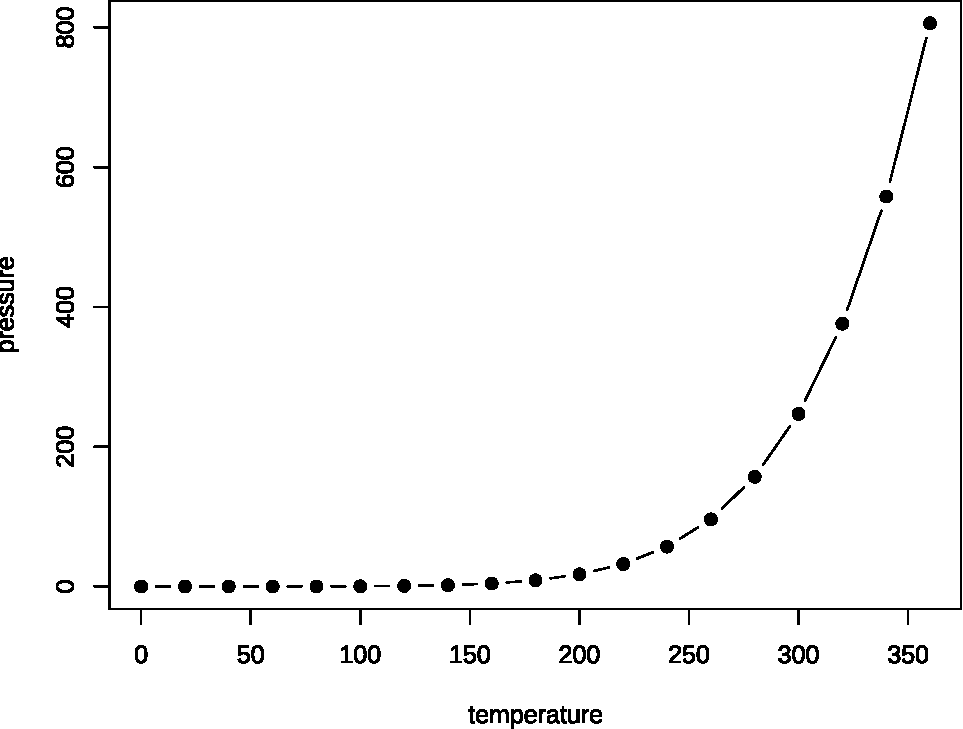
\includegraphics[width=0.8\linewidth]{90-bookdown_files/figure-latex/nice-fig-1} 

}

\caption{Here is a nice figure!}\label{fig:nice-fig}
\end{figure}

Don't miss Table \ref{tab:nice-tab}.

\begin{Shaded}
\begin{Highlighting}[]
\NormalTok{knitr}\SpecialCharTok{::}\FunctionTok{kable}\NormalTok{(}
  \FunctionTok{head}\NormalTok{(pressure, }\DecValTok{10}\NormalTok{), }\AttributeTok{caption =} \StringTok{\textquotesingle{}Here is a nice table!\textquotesingle{}}\NormalTok{,}
  \AttributeTok{booktabs =} \ConstantTok{TRUE}
\NormalTok{)}
\end{Highlighting}
\end{Shaded}

\begin{table}

\caption{\label{tab:nice-tab}Here is a nice table!}
\centering
\begin{tabular}[t]{rr}
\toprule
temperature & pressure\\
\midrule
0 & 0.0002\\
20 & 0.0012\\
40 & 0.0060\\
60 & 0.0300\\
80 & 0.0900\\
\addlinespace
100 & 0.2700\\
120 & 0.7500\\
140 & 1.8500\\
160 & 4.2000\\
180 & 8.8000\\
\bottomrule
\end{tabular}
\end{table}

\hypertarget{parts}{%
\section{Parts}\label{parts}}

You can add parts to organize one or more book chapters together. Parts can be inserted at the top of an .Rmd file, before the first-level chapter heading in that same file.

Add a numbered part: \texttt{\#\ (PART)\ Act\ one\ \{-\}} (followed by \texttt{\#\ A\ chapter})

Add an unnumbered part: \texttt{\#\ (PART\textbackslash{}*)\ Act\ one\ \{-\}} (followed by \texttt{\#\ A\ chapter})

Add an appendix as a special kind of un-numbered part: \texttt{\#\ (APPENDIX)\ Other\ stuff\ \{-\}} (followed by \texttt{\#\ A\ chapter}). Chapters in an appendix are prepended with letters instead of numbers.

\hypertarget{footnotes-and-citations}{%
\section{Footnotes and citations}\label{footnotes-and-citations}}

\hypertarget{footnotes}{%
\subsection{Footnotes}\label{footnotes}}

Footnotes are put inside the square brackets after a caret \texttt{\^{}{[}{]}}. Like this one \footnote{This is a footnote.}.

\hypertarget{citations}{%
\subsection{Citations}\label{citations}}

Reference items in your bibliography file(s) using \texttt{@key}.

For example, we are using the \textbf{bookdown} package \citep{R-bookdown} (check out the last code chunk in index.Rmd to see how this citation key was added) in this sample book, which was built on top of R Markdown and \textbf{knitr} \citep{xie2015} (this citation was added manually in an external file book.bib).
Note that the \texttt{.bib} files need to be listed in the index.Rmd with the YAML \texttt{bibliography} key.

The \texttt{bs4\_book} theme makes footnotes appear inline when you click on them. In this example book, we added \texttt{csl:\ chicago-fullnote-bibliography.csl} to the \texttt{index.Rmd} YAML, and include the \texttt{.csl} file. To download a new style, we recommend: \url{https://www.zotero.org/styles/}

The RStudio Visual Markdown Editor can also make it easier to insert citations: \url{https://rstudio.github.io/visual-markdown-editing/\#/citations}

\hypertarget{blocks}{%
\section{Blocks}\label{blocks}}

\hypertarget{equations}{%
\subsection{Equations}\label{equations}}

Here is an equation.

\begin{equation} 
  f\left(k\right) = \binom{n}{k} p^k\left(1-p\right)^{n-k}
  \label{eq:binom}
\end{equation}

You may refer to using \texttt{\textbackslash{}@ref(eq:binom)}, like see Equation \eqref{eq:binom}.

\hypertarget{theorems-and-proofs}{%
\subsection{Theorems and proofs}\label{theorems-and-proofs}}

Labeled theorems can be referenced in text using \texttt{\textbackslash{}@ref(thm:tri)}, for example, check out this smart theorem \ref{thm:tri}.

\begin{theorem}
\protect\hypertarget{thm:tri}{}\label{thm:tri}For a right triangle, if \(c\) denotes the \emph{length} of the hypotenuse
and \(a\) and \(b\) denote the lengths of the \textbf{other} two sides, we have
\[a^2 + b^2 = c^2\]
\end{theorem}

Read more here \url{https://bookdown.org/yihui/bookdown/markdown-extensions-by-bookdown.html}.

\hypertarget{callout-blocks}{%
\subsection{Callout blocks}\label{callout-blocks}}

The \texttt{bs4\_book} theme also includes special callout blocks, like this \texttt{.rmdnote}.

You can use \textbf{markdown} inside a block.

\begin{Shaded}
\begin{Highlighting}[]
\FunctionTok{head}\NormalTok{(beaver1, }\AttributeTok{n =} \DecValTok{5}\NormalTok{)}
\CommentTok{\#\textgreater{}   day time  temp activ}
\CommentTok{\#\textgreater{} 1 346  840 36.33     0}
\CommentTok{\#\textgreater{} 2 346  850 36.34     0}
\CommentTok{\#\textgreater{} 3 346  900 36.35     0}
\CommentTok{\#\textgreater{} 4 346  910 36.42     0}
\CommentTok{\#\textgreater{} 5 346  920 36.55     0}
\end{Highlighting}
\end{Shaded}

It is up to the user to define the appearance of these blocks for LaTeX output.

You may also use: \texttt{.rmdcaution}, \texttt{.rmdimportant}, \texttt{.rmdtip}, or \texttt{.rmdwarning} as the block name.

The R Markdown Cookbook provides more help on how to use custom blocks to design your own callouts: \url{https://bookdown.org/yihui/rmarkdown-cookbook/custom-blocks.html}

\hypertarget{sharing-your-book}{%
\section{Sharing your book}\label{sharing-your-book}}

\hypertarget{publishing}{%
\subsection{Publishing}\label{publishing}}

HTML books can be published online, see: \url{https://bookdown.org/yihui/bookdown/publishing.html}

\hypertarget{pages}{%
\subsection{404 pages}\label{pages}}

By default, users will be directed to a 404 page if they try to access a webpage that cannot be found. If you'd like to customize your 404 page instead of using the default, you may add either a \texttt{\_404.Rmd} or \texttt{\_404.md} file to your project root and use code and/or Markdown syntax.

\hypertarget{metadata-for-sharing}{%
\subsection{Metadata for sharing}\label{metadata-for-sharing}}

Bookdown HTML books will provide HTML metadata for social sharing on platforms like Twitter, Facebook, and LinkedIn, using information you provide in the \texttt{index.Rmd} YAML. To setup, set the \texttt{url} for your book and the path to your \texttt{cover-image} file. Your book's \texttt{title} and \texttt{description} are also used.

This \texttt{bs4\_book} provides enhanced metadata for social sharing, so that each chapter shared will have a unique description, auto-generated based on the content.

Specify your book's source repository on GitHub as the \texttt{repo} in the \texttt{\_output.yml} file, which allows users to view each chapter's source file or suggest an edit. Read more about the features of this output format here:

\url{https://pkgs.rstudio.com/bookdown/reference/bs4_book.html}

Or use:

\begin{Shaded}
\begin{Highlighting}[]
\NormalTok{?bookdown}\SpecialCharTok{::}\NormalTok{bs4\_book}
\end{Highlighting}
\end{Shaded}


  \bibliography{book.bib,packages.bib}

\end{document}
